\section{Analyse}
\subsection{Was ist ein Spiel?}
\subsection{Lernen durch Videospiele}
Computerspiele leiden unter vielen schlechten Vorurteilen. Ihnen wird eine Steigerung der Aggressivität, eine Vereinsamung oder das Verdummen der Spieler angelastet. Studien widerlegen diese Vorurteile vehement \cite{psylex.de2012}. Entgegengesetzt dazu weisen einige Videospiele sogar Lerneffekte auf \cite{paradisiredaktion2010}. Doch wie genau lernt man und was wird vermittelt? Um dieser Frage nach zu kommen werden einige Spiele genauer betrachtet, dessen Inhalte analysiert und Lernkompetenzen aufgezeigt. 

\subsubsection[Age of Empires]{Age of Empires\footnote{Dieser Abschnitt wird an mehreren Stellen von der Quelle \cite{bundeszentralefuerpolitischebildung2005} referenziert.}}
Eines der betrachteten Spiele ist "{}Age of Empires"{}. Age of Empires ist ein Echtzeit-Strategiespiel, welches sehr gute Grafik und Animationen aufweist. Das Ziel ist es, alle gegnerischen Völker auszulöschen und dabei das Überleben des eigenen Volkes sicherzustellen. Um dieses Ziel zu erreichen, muss ein Imperium erschaffen werden, welches eine ausgeklügelte Infrastruktur und Militärwesen besitzt. Dazu wird eine Vielzahl unterschiedlicher Rohstoffe benötigt, die für die Erstellung der verschiedenen Gebäude, Schiffe und Soldatentypen notwendig sind. Das Ressourcenmanagement ist daher ein essentieller Bestandteil des Spielgeschehens.

Dem Spieler stehen verschiedenste Handlungs- und Entscheidungsmöglichkeiten zur Verfügung. Diese fordern ihn in taktischer und strategischer Disziplin heraus. Aus diesem Grund benötigt dieser eine komplexe denkerische Fähigkeit, um abschätzen zu können, welche Schritte für das eigene Überleben und die Auslöschung des Feindes notwendig sind. Daneben muss er in der Lage sein die Spielsituation zu erfassen und die Strategie des Gegners in die eigene Vorgehensweise einzuberechnen. Zuzüglich sind Stressbewältigung und Reaktionsgeschwindigkeit von großer Bedeutung, der auf dem "{}Realtime-Modus"{} zurückzuführen ist. 

Die meisten Spiele vom Genre Echtzeit-Strategie weisen eine Levelstruktur auf. Mit zunehmenden Levelfortschritts werden die Anforderungen an den Spieler vielfältiger und komplexer. Aufgrund dessen wird der Denkprozess des Spielers angeregt. Neue Methoden und Strategien müssen ausgebildet werden, um das Ziel zu erreichen. Spieler, die bereits Erfahrungen mit diesem Genre gesammelt haben, konnten nachweislich besser Probleme lösen als unerfahrene Spieler. Außerdem waren sie besser in der Lage neue Probleme zu erkennen und diese zu verarbeiten. Die erfahrenere Gruppe der Spieler erkannten Zusammenhänge zwischen den einzelnen Spielelementen schneller und legten Prioritäten, zum Beispiel auf den Ausbau der Stadt. Die Unerfahrenden testeten die unterschiedlichen Elemente aus. Erst beim wiederholten Versuch des selben Levels konnte es erfolgreich abgeschlossen werden. Das wurde durch das Erkennen der Zusammenhänge der unterschiedlichen Spielelemente erreicht.

Der Spieler muss in Age of Empires unterschiedliche Probleme lösen. Darunter zählt ein ausgeklügeltes Ressourcenmanagement, um die verschiedenen Gebäude- und Soldatentypen ausbilden zu können. Darüber hinaus müssen im fortgeschrittenen Levelabschnitt neue Taktiken und Handlungsschemata ausgebildet werden, um die komplexer werdenden Aufgaben zu erfüllen und den Feind auszulöschen. Darüber hinaus wird die allgemeine Wahrnehmung geschult. Das zeigt sich durch frühzeitige Erkennung der feindlichen Aktivitäten, woraus sich wiederum eine erhöhte Reaktionsgeschwindigkeit ableitet, die zum Einleiten der Gegenmaßnahmen notwendig sind. 

Ein Lerneffekt ist nach Zusammenfassung dieser Aspekte in Age of Empires nachgewiesen.

\subsubsection{Counter Strike}
Ein weiteres untersuchtes Spiel ist "{}Counter Strike"{}. Hierbei handelt es sich um ein 3D Online-Taktik-Shooter, wo eine Terrorristengruppen gegen eine Antiterroreinheit kämpft. Das Ziel ist es, das jeweils gegnerische Team vollständig auszulöschen oder die gesetzte Bombe der Terrorristen zu entschärfen bzw. die Geiseln zu retten. Zur Verfügung steht ein großes Repertoire an Gewehren, Pistolen, Messer, aber auch Schutzkleidung, welches mit Geld erworben wird.

Um das Ziel des Spiels zu erreichen muss sich der Spieler bewegen können. Das ist allerdings nur möglich, wenn er sich in einem 3-Dreidimensionalem Raum zurechtfinden kann. Dafür wird die räumliche Vorstellungskraft benötigt, die sich während des Spielens verbessert.\cite{christianstoecker2004} Objekte und Hindernisse werden mit zunehmender Spielerfahrung leichter überwunden, auch die Schätzungen von Entfernungen sind präziser. Vor allem die kognitive Wahrnehmung der Umgebung, insbesondere der bewegte Objekten werden trainiert.\cite{frankstoewer2003} 

Neben der Bewegung ist auch das Zielen ein ausschlaggebender Bestandteil des Spielgeschehens. Die Maus, welche direkt mit der Zielvorrichtung gekoppelt ist, muss zum Gegner gesteuert werden. Dieses Verhalten fordert eine ausgesprochen hohe Hand-Augen-Koordination, da sich der Gegner immer an einer anderen Position befindet und zusätzlich bewegt. In Abhängigkeit der Lokation des Gegners (Das Auge nimmt den Gegner als Reiz auf.) muss die Maus in Richtung des Ziels gesteuert werden (Die Hand steuert die Maus zur gewünschten Stelle, sodass sich der Feind im Bildzentrum befindet.). Durch wiederholten Spielen verbessert sich die Hand-Augen-Koordination, welche grundlegender Bestandteil des Spielvergnügens darstellt.\cite{mathias2014} Neben der Hand-Augen-Koordination ist auch dort die räumliche Vorstellungskraft wesentlicher Bestandteil, weil sie das Anvisieren erst ermöglicht. 

Feinde können sich blitzschnell um Ecken bewegen und den Spieler erschießen. Um das zu verhindern kann sich der Spieler hinter Objekte verstecken oder schnellstmöglich den Feind auslöschen. Das ist allerdings nur möglich, wenn eine hohe Reaktionsgeschwindigkeit besteht. Unerfahrene Spieler weisen ein langsameres Reaktionsverhalten auf \cite{jankloft2013} und werden häufiger von der gegnerischen Fraktion getötet. Erfahrene Spieler, welche bereits viel Spielzeit aufgebracht haben, zeigen ein deutlich erhöhtes Reaktionsverhalten\cite{stern.de2010} und können extrem schnell die richtigen Entscheidungen treffen, die ihr Überleben sichern\cite{samiskalli2010}\cite{cib/dapd2010}.

Entscheidende Faktoren, die zur Verbesserung der Reaktion beitragen, sind geschulte visuelle und akustische Aufmerksamkeit. Die visuelle Aufmerksamkeit wird hauptsächlich durch die Bewegung andere Spieler verursacht. Das liegt an der evolutionär bedingten Wahrnehmung des Auges, welches sofortige Aufmerksamkeit zum bewegten Objekt verursacht \cite{juliagross2011}. Neben der visuellen kann ebenfalls die akustische Wahrnehmung geschult werden. Personen, die dieses Spiel mit Ton spielen, haben die Möglichkeit andere Charaktere zu hören. Dabei sind Explosionen, Schüsse, aber auch die schnellen Bewegungen (Rennen des Charakters) eines Spielers wahrzunehmen. Diese Erkenntnis kann genutzt werden, um den Feind zu überraschen oder um Taktiken auszuarbeiten.

Counter Strike ist ein Multiplayer-Spiel. Das bedeutet, es treffen mehrere reale Personen aufeinander, die ein Team bilden. Ein erfolgreiches Abschließen der Mission kann durch Teamarbeit und koordiniertes Agieren der Spieler vereinfacht werden. Das erfordert Kommunikationen zwischen den Teammitgliedern, welche in einem Chat oder über einem Sprachdienst abgehalten wird. Spieler, die oft einen der Dienste in Anspruch nehmen, schulen somit ihre kommunikative Fähigkeiten\cite{achimkleinundtimokucza2004} und verbessern unter Umständen ihre Fremdsprachenkenntnisse. \cite{thomaswagner2011}

Der Spieler muss in Counter Strike die gegnerische Fraktion vollständig auslöschen oder die Nebenmission erfüllen. Um diese Ziele zu erreichen, müssen unterschiedliche Fähigkeiten und Kompetenzen genutzt werden. Einerseits ist eine umfangreiche Hand-Augen-Koordination notwendig, damit der Feind anvisiert werden kann. Darüber hinaus ist eine ausgebildete räumliche Vorstellungskraft unverzichtbar, welche die Bewegung, aber auch das Zielen ermöglicht. Ein trainiertes Reaktionsverhalten ist ebenfalls essentiell. Es dient zum eigenen Schutz, aber auch um blitzschnell zu reagieren zu können, um den Feind auszulöschen. Unterstützt wird diese Fähigkeit durch eine gute visuelle und akustische Wahrnehmung, welche sich durch zunehmender Spielerfahrung sensibilisiert.

Nach Zusammenfassung dieser Aspekte ist auch in Counter Strike ein Lernprozess nachweisbar.

\subsubsection{Flappy Bird}
Das zuletzt untersuche Spiel ist ein Mobile Game, welches zum Genre Jump $'$n Run zählt. Hierbei handelt es sich um das bekannte Spiel "{}Flappy Bird"{}. Flappy Bird ist ein 2D-Spiel, welches eine ähnliche Grafik wie Super Mario World aufweist. Das Ziel des Spiels ist es, einen Vogel zwischen zwei Röhren zu führen und möglichst viele Punkte zu sammeln. Die Welt bewegt sich dabei von rechts nach links.

Um das Spiel zu starten muss der Bildschirm berührt werden, worauf hin der Vogel nach unten fällt. Durch erneutes berühren des Touchscreens "springt" der Vogel nach oben, um kurze Zeit später wieder nach unten zu fallen. Um diese Aufgabe zu erfüllen ist eine große Hand-Augen-Koordination notwendig, da sich der Vogel im richtigen Zeitpunkt nach oben bewegen muss. Berührt dieser eines der Hindernisse so ist das Spiel beendet und es kann erneut begonnen werden.

Das Mobile Spiel Flappy Bird weist lediglich einen lehrenden Aspekt auf. Diese beschränkt sich auf die Ausbildung der Hand-Augen-Koordination, da sie der einzig wichtige Aspekt darstellt.\cite{patrickbaalmann2014}

\subsubsection{Lernen durch Videospiele: Fazit}
"{}Age of Empires"{}, "{}Counter Strike"{} und "{}Flappy Bird"{} sind Spiele, die aus unterschiedliche Genres stammen. Sie stellen verschiedene Anforderungen an den Spieler, verwenden differenzierte Spielprinzipien und weisen verschiedenartige Ziele auf. Doch sie besitzen eine Gemeinsamkeit: den Spieler zu motivieren die Feinde zu vernichten, möglichst viele Punkte oder Erfolge zu sammeln. Diese Motivation veranlasst den Spieler das Spiel erneut zu spielen, sodass dieser mehr Punkte sammelt und sich selbst übertreffen. Direktes Feedback vom Spiel, z.B. das Erhalten von Punkte in Flappy Bird, spornt an, noch mehr Punkte zu erreichen. 

Durch das Wiederholen der Spieltätigkeit mit dem Ziel besser zu sein als vorher oder den Gegner zu bezwingen, werden die einzelnen Kompetenzen, wie analytisches Denken, Reaktionsgeschwindigkeit, visuelle und akustische Wahrnehmung geschult und stetig verbessert. Auch das Zurechtfinden in einem 3D-Raum, die Hand-Augen-Koordination oder soziale Qualitäten, wie Teamfähigkeit oder Kommunikation in einer Gruppe werden hochwertiger und gefördert. 

Obwohl alle der oben genannten Spiele verschiedene Genres bedienen und Tätigkeiten abverlangen, haben diese doch eines gemeinsam: sie vermitteln alle eine spezielle Art von Wissen, die sich direkt auf unsere Fähigkeiten auswirken. 

\subsection{Wahl der Spielart}
\TODO{Hier kommt Text warum wir uns für das Lichtspiel entschieden haben}
\TODO{Wie sind wir auf die Idee gekommen?}
\TODO{Idee wurde unterstützt durch das Spiel God of Lights}

\subsection{Spielgenre}
\TODO{Hier kommt Text warum wir uns für das Genre entschieden haben}

\subsection{Spielkonzept}
\subsubsection{Grundidee}
Die Grundidee dieses Spiels ist es, einen Weltenbaum mit Licht zu versorgen und dadurch wachsen zu lassen. Dafür muss der Lichtstrahl durch unterschiedliche Puzzle-Rätsel ans Ziel geleitet werden. Um das Ziel zu erreichen muss mit unterschiedlichen Objekten interagiert werden. Mit zunehmenden Levelfortschritts müssen komplexere Objekte verwendet werden. Im Laufe des Spiels entwickelt sich der Samen zum Weltenbaum.

\subsubsection{Darstellung des Spiels}
Das Spiel soll in einem Comichaften 2.5D Stil dargestellt werden. Dabei sollen die Grafiken in einem tristen Schwarzweiß mit farbigen Hintergrund verwendet werden. Nach dem Erleuchten des einzelnen Gebiets sollen diese in bunten Farben erstrahlen. Die einzelnen Szenarien und Level befinden sich in Höhlen, auf Wiesen und im Wald.

\TODO {HIER GRAFIKELEMENTE AUFZEIGEN}


Die Idee und Darstellung des Spiels wird im Kapitel \ref{ganmeDesignDoku} genauer erläutert.

\subsection{Engine}
\subsubsection{Was ist eine Engine?}
Eine Spielengine ist der „Motor“ hinter dem eigentlichen Spiel und wird als Framework bzw. Entwicklungsumgebung angeboten. Die Engine steuert den gesamten Spielverlauf und ist ebenfalls für die visuelle Darstellung sowie die Berechnung der Physik verantwortlich. In folgenden Kapitel werden mehrere unterschiedliche Engines verglichen und anhand unserer Anforderungen eine passende ausgewählt. 

\subsubsection{\ac{UE4} vs \ac{U5} vs \ac{BGE}}[Test]
Da es sich bei dem Spiel um ein Puzzle und Logikspiel handelt, mit welchem auch Lerninhalte vermittelt werden sollen, werden die Casualgamer und Kinder als Zielgruppe ausgewählt. Um diese Zielgruppe zu erreichen muss die entsprechende Plattform gewählt werden, welche eine möglichst große Anzahl der Zielgruppe abdeckt. Dafür eignen sich besonders Mobilgeräte, da diese heutzutage fast jeder besitzt und auch darauf Spiele spielt.  \\

\textbf{Plattformen:}\\
Alle zu vergleichenden Engines unterstützen Windows und Linux Rechner sowie MAC OS X. Zusätzlich sind \ac{U5} und \ac{UE4} mit den gängigen mobilen Betriebssystemen Android und Apples IOS kompatibel und erlauben auch die Entwicklung an Microsofts und Sonys aktuellen Konsolen Xbox One und Playstation 4. Doch auch ganz neue Betriebssysteme und Technologien wie VR und Steam OS werden von Haus aus unterstützt.

\begin{table}[H]
\centering
\renewcommand{\arraystretch}{1.5}
\begin{tabular}{lp{14.5cm}}
\ac{U5}:  & Zusätzlich unterstützt \ac{U5} weitere mobile Plattformen wie Windows Phone 8, Tizen und die Playstation Vita. Auch für TV Geräte wie Android TV oder Samsung Smart TV können Spiele mit der \ac{U5} Engine entwickelt und gespielt werden. Im Gegensatz zu \ac{UE4} ist \ac{U5} auch mit älterer Konsolenhardware, wie der Xbox 360 und der Wii U kompatibel. Aber auch Webanwendung mit WebGL oder dem Unity Web Player können erstellt werden. \\

\ac{UE4}: & \ac{UE4} hat den weiteren Vorteil dass auch HTML5 unterstützt wird. \\

\ac{BGE}:     & Mit \ac{BGE} ist auch die Entwicklung für Mobilgeräte mit Android Betriebssystem möglich. Voraussetzung dafür ist, dass auf dem Mobilgerät Android \ac{BGE} Player GSOC 2012 installiert ist. 
\end{tabular}
\end{table}

Wie man sehen kann erfüllen alle Engines die Voraussetzung mit mobilen Geräten kompatibel zu sein. Da es sich bei diesem Projekt um ein Studienprojekt handelt, sollten sich auch die Lizenzgebühren und die laufenden Kosten im unteren Bereich befinden. Womit der nächste Kritikpunkt unseres Vergleiches die Lizenzierung sowie die Kosten betreffen. \\



\textbf{Lizenz und Kosten:}
\begin{table}[H]
\centering
\renewcommand{\arraystretch}{1.5}
\begin{tabular}{lp{14.5cm}}
\ac{U5}: & \ac{U5} kann als zwei verschiedenen Arten erworben werden. Die Personal Edition steht dabei Kostenfrei zur Verfügung und kann mit vollen Featureumfang der Engine erworben werden. Zusätzlich gibt es die Pro Variante, welche pro Release gezahlt oder durch einen Monatlichen Beitrag erworben werden kann. Diese Edition bietet weitere Möglichkeiten effizienter zu arbeiten, wie zum Beispiel durch eine Teamlizenz. Weiterhin gibt es in der Pro Variante mehr Möglichkeiten sein erstelltes Spiel durch eigene Bootanimationen u.ä. zu gestalten.\\
UE4:& Die Unreal Engine ist seit März 2015 kostenfrei zu erwerben und kann bedingungslos verwendet werden. Falls beim Verkauf des entwickelten Spiels mehr als 3000 Dollar Umsatz erwirtschaftet wird, hält sich Epic Games (die Entwickler der Unreal Engine) das Recht vor, 5 Prozent des Umsatzes als Lizenzgebühr zu  verlangen.\\
\ac{BGE}: & \ac{BGE} ist eine freie Software  und kann uneingeschränkt genutzt, verändert und die erstellten Produkte verkauft werden.
\end{tabular}
\end{table}

Alle der genannten Engines sind für dieses Projekt ohne Kosten und Lizenzgebühren nutzbar und eignen sich für diese Arbeit.
Für dieses Projekt ist nicht nur eine Kostenübersicht notwendig, sondern sollte auch ein guter Einstieg durch Tutorials/ Literatur/Dokumentationen ermöglicht werden. \\

\textbf{Erlernbarkeit:}\\
Alle der besagten Engines besitzen eine sehr gute Dokumentationen. Durch die visuelle Unterstützung durch Screenshots von der \ac{UE4}  wird die ohnehin gut beschriebene Dokumentation noch hochwertiger. Jede der Engines besitzt eine große Community, wodurch auch sehr viele Tutorials und Wiki Einträge vorhanden sind. Zusätzlich gibt es eine  vielzahl an  Anleitungen von professionellen Entwicklern, die ihr Wissen allen Benutzergruppen (Neuling/Fortgeschritten/Experte) zur Verfügung stellen. Weiterhin gibt es eine große Auswahl an Literatur für den Einstieg mit \ac{U5} und \ac{BGE}. Da sich \ac{UE4} noch in der Entwicklung befindet, ist die Literaturauswahl eingeschränkt (vor allem in der deutschen Sprache).

Alle der Engines haben eine große Community und bieten auch sehr viele gute einsteigerfreundliche Möglichkeiten an. 
Um eine gute Einarbeitung zu ermöglichen und mit der Engine effizient zu arbeiten spielt auch die Nutzbarkeit und die Komplexität des Interface eine Rolle.\\

\textbf{Nutzbarkeit:}\\
Die einzelnen Interfaces unterscheiden sich nur leicht voneinander und sind mit beweglichen/skalierbaren Fenstern flexibel anpassbar. Die einzelnen Entwicklungsumgebungen können auf allen gängigen Betriebssystemen eingesetzt werden.
\begin{table}[H]
\centering
\begin{tabular}{lp{14.5cm}}
\ac{UE4}:& 
Das \ac{UE4} Interface ist komplexer als das von \ac{U5}. Dieses ist eher für Benutzer mit Erfahrung geeignet, da es den Einstieg etwas erschwert. Darüber hinaus beansprucht \ac{UE4} mehr Zeit für das Ausführen von Aufgaben, wie Speichern des Projekts oder Importieren von Assets. Zudem kommt hinzu, dass \ac{UE4} eine sehr hardwarelastige Engine ist, welche mehr Ressourcen des Endgerätes verwendet, als die anderen Engines.\\
\ac{U5}:&
\ac{U5} hat den Vorteil, dass es sehr schnell reagiert und auch kleinere Aufgaben sehr schnell abarbeitet.\\  
\ac{BGE}:&
Das \ac{BGE} Interface ist, wie auch das \ac{UE4} Interface, komplexer und benötigt mehr Einarbeitungszeit.
\end{tabular}
\end{table}
Da das Projekt für Mobilgeräte entwickelt wird, welche nicht immer mit der aktueller Hardware ausgestattet ist, eignet sich gerade aus dem Aspekt der Nutzbarkeit die Unity Engine besonders gut.
Dieses Projekt ist für ein Team dieser Größe nur sehr schwer realisierbar, daher ist die Unterstützung aus der Community wichtig. Die Engines sollten bestimmte Assets zur Verfügung stellen und auch eine möglichst günstige und vielfältige Auswahl anbieten.\\

\textbf{Unterstützung:}\\
Durch sogenannte Assets kann man sich bereits erstellte Projektteile herunterladen und in seiner eigenen Arbeit verwenden. Diese können einfache Scripte bis hin zu komplexe Grafikelemente oder Animationen sein. Hierbei stehen kostenfreie sowie kostenpflichtige zur Verfügung. Da \ac{UE4} relativ neu ist, ist auch die Auswahl kleiner als im Unitystore. Nichtsdestotrotz kommen täglich neue Inhalte hinzu. \ac{BGE} stellt aus ihrer Community eine umfangreiche Auswahl aus allerlei verschiedensten Bereichen von Assets bereit. Diese werden meistens kostenlos angeboten und enthalten oft eine vollständige Anleitung wie dieses Asset erstellt wurde. Bei \ac{U5} sind ebenfalls sehr viele Assets kostenlos. Die kostenpflichtigen fallen in der Regel günstiger aus, als die von \ac{UE4}.

Die Auswahl ist bei allen drei Engines riesig. Jedoch ist durch die längere Etablierung der \ac{U5} und \ac{BGE} eine deutlich größere Auswahlmöglichkeit vorhanden. Diese sind meist günstiger oder sogar komplett Kostenfrei zu erwerben.\\

\textbf{Physik:}\\
Durch Physik entsteht der Eindruck in jeder einzelnen Szene des Spiels interagieren zu können. Der Spieler erhält dadurch ein direktes Feedback. Eine korrekte Physik gibt dem Spieler das Gefühl in die Spielewelt "eintauchen" zu können. Diese kann dadurch als real wahrgenommen werden. Gerade für ein Spiel das mit physikalischen Grundprinzipien arbeitet, ist dies ein wichtiger Bestandteil den man bei der Entscheidung berücksichtigen sollte. 
\begin{table}[H]
\centering
\begin{tabular}{lp{14.5cm}}

\ac{U5}: &
\ac{U5} basiert für physikalische Berechnungen auf der PhysX Engine, welche für 3D Modellierungen verwendet wird. Für 2D Projekte nutzt \ac{U5} die Box 2D Engine. Diese ist Open Source und ist in \ac{U5} bereits nativ implementiert. Box 2D eignet sich speziell für Rigidbody2D Objekte, mit dem auch \ac{U5} arbeitet.\\
\ac{UE4}:& Die Physik in \ac{UE4} basiert ebenfalls auf der PhysX Engine von Nvidia. Diese ermöglicht es, korrektes physikalisches Kollissionsverhalten zwischen mehreren 3D Objekten zu berechnen und darzustellen. Für 2D Projekte verwendet \ac{UE4} die eigen entwickelte Paper2D-Engine. \\

\ac{BGE}:&
Bei \ac{BGE} kommt für die Physik die Bullet Physik Engine zum Einsatz. Diese ermöglicht die korrekte physikalische Berechnungen für Partikelsysteme, starre Körper sowie Flüssigkeiten, Kraftfelder und Gravitation.
\end{tabular}
\end{table}


\textbf{Grafik:}\\
Die Grafik eines Spiels bestärkt die Immersion und sorgt für eine optische Darstellung des Spiels. Dieses Spiel soll im 2.5D stilisiert werden und die Engine sollte entsprechende Grafiken dazu ermöglichen.
\begin{table}[H]
\centering
\begin{tabular}{lp{14.5cm}}

\ac{UE4}:&
Die \ac{UE4} verwendet für das Rendern der Grafiken ein eigenes Rendering System, welches auf OpenGL basiert. \ac{UE4} verwendet eine neue DirectX11-Pipeline, welche es dem Grafikprozessor erlaubt Änderungen von Beleuchtungen und Shading-Effekte im Nachhinein vorzunehmen.\\
\ac{U5}: &
\ac{U5} unterstützt OpenGL und Direct3D. Welches Shadingverfahren dabei zum Einsatz kommt hängt dabei von der  Zielplattform ab. Die integrierten Beleuchtungsmodelle können mit selbsterstellten Shadern erweitert oder modifiziert werden.\\
\ac{BGE}:&
Blender ist eine 3D Software zum Erstellen von Animationen oder Modellen, welche auf DirectX und OpenGL basiert. Zudem ist eine eigen entwickelte Game-Engine integriert. Der Unterschied zwischen dem "normalen Modus" und \ac{BGE} ist der Render-Vorgang. In der Game Engine wird jede Szene einzeln und in Echtzeit gerendert. Im Gegensatz dazu rendert der normale Modus die Modelle/Bilder/Animationen im voraus und sind nach dem Vorgang nicht mehr veränderbar.
\end{tabular}
\end{table}
Dadurch dass die \ac{BGE} nicht ohne weiteres 2D Projekt unterstützt, ist \ac{U5} oder \ac{UE4} die bessere Variante.
Die Entwicklungssprache der Engine ist nur zweitrangig, jedoch sollte diese verglichen werden, um zum Beispiel Einarbeitungszeiten zu verkürzen.\\

\textbf{Scriptsprachen:}
\begin{table}[H]
\centering
\begin{tabular}{lp{14.5cm}}
\ac{UE4}:&
\ac{UE4} setzt bei der Erstellung der Spiele auf C++  und den sogenannten Blueprint Scripting. Mit diesen ist es möglich Abläufe von bestimmten Aktionen /Situationen/Abläufen durch visuelle Darstellung durch Modelle zu definieren und Erstellen.\\
\ac{U5}:&
\ac{U5} verwendet als Scriptsprachen C\#, Boo und Unityscript, welches an Javascript anlehnt und aufbaut. Man ist nicht auf eine Sprache begrenzt und es ist frei, welche man für die Entwicklung verwendet. \ac{U5} bietet die Möglichkeit der visuellen Scripte, wie \ac{UE4} standardmäßig, nicht an. Erweiterungen dafür können aber im Assetstore erworben werden.\\

\ac{BGE}:&
Für die Entwicklung mit der \ac{BGE} wird ein Logikeditor verwendet, welcher Logikbausteine für Interaktionen, Animationen und Situationen anbietet. Diese sind durch C++ oder Python Scripte erweiterbar.

\end{tabular}
\end{table}

\subsubsection{Fazit}
Alle oben genannten Kriterien wurden beachtet, um sich für eine Engine zu entscheiden, die für das eigene Spiel eingesetzt werden soll. Da kaum bis keine Erfahrung mit dem Umgang von Engines besteht, ist ein guter Einstieg und die Möglichkeiten sich durch Tutorials und Literatur einzuarbeiten sehr wichtig. Zusätzlich wurde sich für ein 2.5D Stil der Grafik entschieden, welches mit Lichtphysik interagiert und auf mobilen Plattformen unterstützt wird. Durch die geringe Leistung vieler Geräte ist es wichtig auf die Performance der Geräte zu achten. Diese Voraussetzungen und die Erarbeitung der einzelnen Unterschiede machten schnell klar, dass sich \ac{U5} für dieses Projekt am besten eignet. Es bietet eine umfangreiche Möglichkeit der Einarbeitung, einen 2D Rendermodus sowie Physikeffekte, und unterstützt mobile Endgeräte mit leistungsschwacher Hardware. 

\subsection{Konzepte und Formeln aus der Physik}
Innerhalb des Spiels werden mehrere physikalische Gegebenheiten abverlangt. Eines ist die Reflexion. Diese wird verwendet um den Lichtstrahl von Spiegeln reflektieren zu lassen.
\subsubsection{Reflexion}
Im Spiel wird die Reflexion hauptsächlich durch Spiegel hervorgerufen. Hierbei werden physikalische Gesetzmäßigkeiten beachtet, sodass eine korrekte Darstellung des Lichtstrahls sichergestellt ist. Die Reflexion wird im allgemeinen durch das Reflexionsgesetz definiert:
\begin{enumerate}
\item "{}Einfallender Strahl, Einfallslot und reflektierender Strahl liegen in einer Ebene."{}
\item "{}Einfallswinkel und Reflexionswinkel sind gleich groß."{}\cite{baderdorn1980}
\end{enumerate}
Doch was genau bedeutet das?

Der Einfallende Strahl repräsentiert den Lichtstrahl, der auf den Spiegel trifft. Der Reflektierende Strahl zeigt, wie er vom Spiegel zurück geworfen wird. Das Einfallslot ist eine Hilfslinie, welche orthogonal auf der Spiegelfläche, im Auftreffpunkt des Lichtstrahls steht. Das Einfallslot kann als eine Art Zeiger betrachtet werden, da sie bei jeder Verdrehung des Spiegels eine andere Richtung einschlägt und somit die Lage des Spiegels charakterisiert. Der Einfallswinkel ist der Winkel zwischen dem einfallenden Lichtstrahl und dem Einfallslot. Der Reflexionswinkel ist der Winkel zwischen dem Lot und dem reflektiertem Strahl.
\TODO{Aus dem Buch Seite 198-199)}

Die 2. Regel gibt an, dass der Einfalls- und Reflexionswinkel gleich groß sind. Das bedeutet, dass der reflektierte Strahl den selben Winkel aufweist, wie der einfallende Strahl. Verdeutlicht wird dieses Regel durch das Bild in Abbildung \ref{reflecWinkel}.
\begin{figure}[H]
\centering
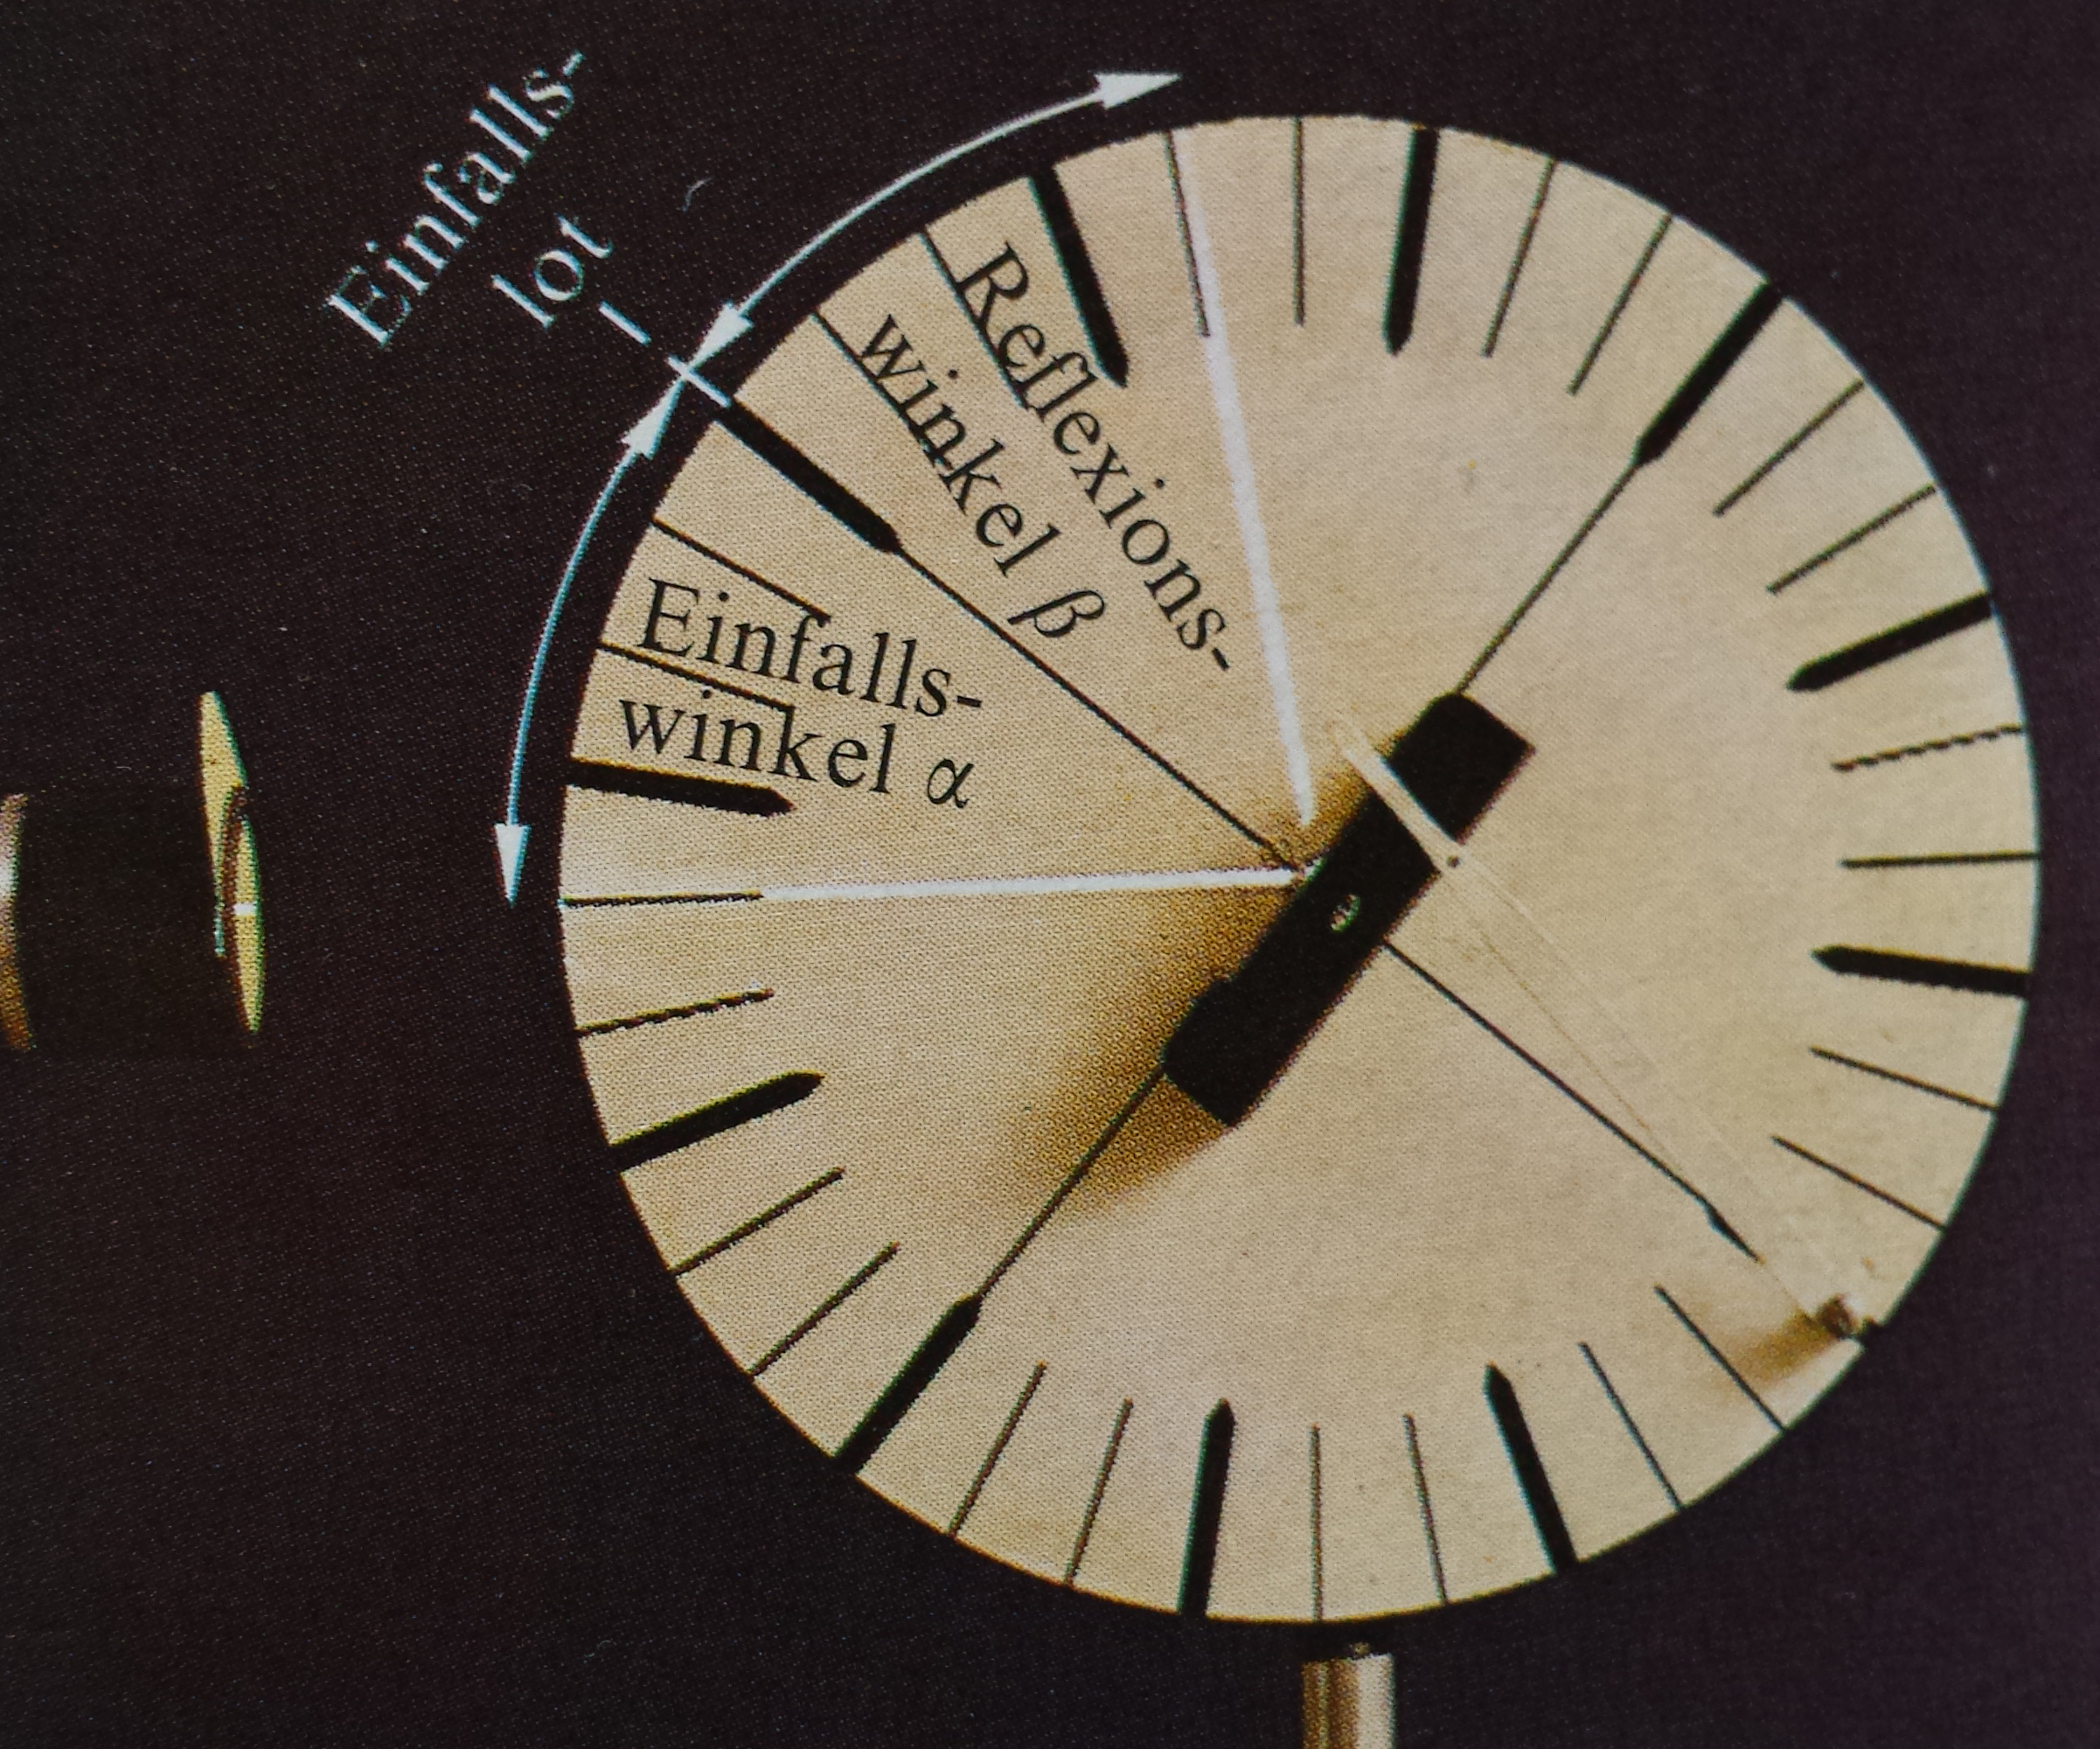
\includegraphics[scale=0.09, center]{res/reflecWinkel.jpg}
\caption{Reflektierender Lichtstrahl}
\label{reflecWinkel}
\end{figure}


\subsubsection{Brechung}

Doch wie können die einzelnen Winkel berechnet werden?\\
Die Bestimmung des Auftrittswinkel $\alpha$ erfolgt ohne größeren Aufwand. Hierfür wird die Vector3.Angle()-Funktion aus Unity herangezogen, welche den Winkel zwischen dem einfallendem Lichtstrahl und dem Lot ermittelt. Die Berechnung des Brechungswinkels ist dahingegen nicht ohne weiteres möglich. Hierfür muss das Snelliussches Brechungsgesetz und der Brechungsindex der unterschiedlichen Materialien bekannt sein. Der Brechungsindex n ist eine physische Größe, die das Verhältnis der Lichtgeschwindigkeit im Vakuum und der Ausbreitungsgeschwindigkeit im Medien angibt. Die allgemeine Formel lautet: $n = \frac{c_0}{c_M}$, wobei $c_0$ die Vakuumlichtgeschwindigkeit und $c_M$ die Geschwindigkeit im Medium darstellt. Eine Beispielrechnung zeigt den Übergang von Luft zu Wasser:
\begin{center}
$n_{Luft\rightarrow Wasser} = \frac{c_{Luft}}{c_{Wasser}} = \frac{300.000\frac{km}{s}}{225.000\frac{km}{s}}$ = 1,33
\end{center}
In der nachfolgenden Tabelle werden die für dieses Projekt notwendigen Stoffe und ihre Brechzahlen dargestellt.

\begin{table}[H]
\centering
\begin{tabular}{l|c}
\multicolumn{1}{c}{Stoff} & \multicolumn{1}{|c}{Brechungsindex n} \\ \hline \hline
Wasser                    & 1.33                               \\ \hline
Glas                      & 1.53                               \\ \hline
Luft                      & 1.00                               \\ \hline
Diamant                   & 2.40                               \\ \hline
Eis                       & 1.31                               
\end{tabular}
\caption{Brechungsindex verschiedener Materialien}
\label{brechungsindex}
\end{table} 

Das Brechungsgesetz weist die folgende Formel auf, woraufhin durch Umformung der Brechungswinkel $\beta$ berechnet werden kann: 
\begin{center}
$\frac{\sin\alpha}{\sin\beta}$ = $\frac{n_2}{n_1}$ $\Rightarrow$ $\beta$ $=$  $\arcsin\frac{\sin\alpha * n_1}{n_2}$
\end{center}
Tritt ein Lichtstrahl in einen Stoff, der eine Höhere Brechzahl aufweist als der Erste ($n_2 > n_1$), dann wird er zur orthogonalen hin gebrochen und $\beta$ ist kleiner als $\alpha$. Tritt jedoch der Strahl von einem Stoff mit einer hoher optischen Dichte in einem mit einer geringeren, so wird er von der orthogonalen weg gebrochen und $\beta$ ist kleiner als $\alpha$. Beim zweiten Fall ist zu beachten, dass $n_1$ die Brechzahl des \textit{optisch dichteren} und $n_2$ die des \textit{dünneren Stoffes} sind. Zur Berechnung und Veranschaulichung des Brechungswinkel müssen nur noch die entsprechenden Werte eingetragen und die Regeln beachtet werden. Dies wird Anhand zweier Beispiele gezeigt.

\begin{enumerate}
\item Beispiel: wenig dichter Stoff in dichter Stoff\\
Gegeben sind die Brechzahlen für Luft $n_1$ = $n_L$ = 1 und Wasser $n_2$ = $n_W$ = 1.33 sowie der Einfallswinkel mit $\alpha$ = 50\degree.
Nun wird in das Snelliussches Brechungsgesetz eingesetzt und der Brechungswinkel berechnet.
\begin{center}
$\frac{\sin\alpha}{\sin\beta}$ = $\frac{n_2}{n_1}$ $\Rightarrow$ $\frac{\sin 50\degree}{\sin\beta}$ = $\frac{1.33}{1}$ $\Rightarrow$ $\beta$ $=$  $\arcsin\frac{\sin 50 * 1}{1.33}$ $\Rightarrow$ $\beta = 35.1\degree$
\end{center}

\item Beispiel: dichter Stoff in wenig dichter Stoff\\
Gegeben sind die Brechzahlen für Luft $n_2$ = $n_L$ = 1 und Glas $n_1$ = $n_G$ = 1.33 sowie der Einfallswinkel mit $\alpha$ = 30\degree.
Nun wird in das Snelliussches Brechungsgesetz eingesetzt und der Brechungswinkel berechnet.
\begin{center}
$\frac{\sin\alpha}{\sin\beta}$ = $\frac{n_2}{n_1}$ $\Rightarrow$ $\frac{\sin 30\degree}{\sin\beta}$ = $\frac{1}{1.53}$ $\Rightarrow$ $\beta$ $=$  $\arcsin\frac{\sin 30 * 1.53}{1}$ $\Rightarrow$ $\beta = 49.9\degree$
\end{center}
\end{enumerate}

$\cos\alpha = \frac{\vec{a} \circ \vec{a}}{|\vec{a}| * |\vec{b}|} \Rightarrow  \alpha = \arccos \frac{\vec{a} \circ \vec{a}}{|\vec{a}| * |\vec{b}|}$


\newpage